\documentclass[10pt,xcolor=svgnames,169]{beamer} %Beamer
\usepackage{palatino} %font type
\usefonttheme{metropolis} %Type of slides
\usefonttheme[onlymath]{serif} %font type Mathematical expressions
\usetheme[progressbar=frametitle,titleformat frame=smallcaps,numbering=counter]{metropolis} %This adds a bar at the beginning of each section.
\useoutertheme[subsection=false]{miniframes} %Circles in the top of each frame, showing the slide of each section you are at

\usepackage{appendixnumberbeamer} %enumerate each slide without counting the appendix
\setbeamercolor{progress bar}{fg=Maroon!70!Coral} %These are the colours of the progress bar. Notice that the names used are the svgnames
\setbeamercolor{title separator}{fg=DarkSalmon} %This is the line colour in the title slide
\setbeamercolor{structure}{fg=black} %Colour of the text of structure, numbers, items, blah. Not the big text.
\setbeamercolor{normal text}{fg=black!87} %Colour of normal text
\setbeamercolor{alerted text}{fg=DarkRed!60!Gainsboro} %Color of the alert box
\setbeamercolor{example text}{fg=Maroon!70!Coral} %Colour of the Example block text


\setbeamercolor{palette primary}{bg=NavyBlue!50!DarkOliveGreen, fg=white} %These are the colours of the background. Being this the main combination and so one. 
\setbeamercolor{palette secondary}{bg=NavyBlue!50!DarkOliveGreen, fg=white}
\setbeamercolor{palette tertiary}{bg=NavyBlue!40!Black, fg= white}
\setbeamercolor{section in toc}{fg=NavyBlue!40!Black} %Color of the text in the table of contents (toc)

%These next packages are the useful for Physics in general, you can add the extras here. 
\usepackage{amsmath,amssymb}
\usepackage{slashed}
\usepackage{cite}
\usepackage{relsize}
\usepackage{caption}
\usepackage{subcaption}
\usepackage{multicol}
\usepackage{booktabs}
\usepackage[scale=2]{ccicons}
\usepackage{pgfplots}
\usepgfplotslibrary{dateplot}
\usepackage{geometry}
\usepackage{xspace}
\newcommand{\themename}{\textbf{\textsc{bluetemp}\xspace}}%metropolis}}\xspace}

\newcommand{\VTNote}[1]{\todo{VT: #1}}
\newcommand{\prob}{\mathit{Pr}}
\newcommand{\U}{\mathcal{U}}
\newcommand{\Lap}{\mathit{Lap}}
\theoremstyle{definition}
\newtheorem{defn}{Definition}

\theoremstyle{theorem}
%\newtheorem{lemma}{Lemma}
\newtheorem{prop}{Proposition}

\title[]{Privacy in the Right To Ask project}

\author[Name]{Vanessa Teague\inst{$\dagger$} and Chris Culnane}

%\author[]{}

\date[]{\today}


%\subtitle{Influence Without Surveillance}
\institute[uni]{\inst{$\dagger$} vanessa@thinkingcybersecurity.com and the ANU \\ \\ \url{https://github.com/RightToAskOrg}\\  \\ With thanks to these contributors: Andrew Conway, Rosey Conway, Charmaine Chew, Ishan Goyal, Matt Lefurge, Chuanyuan Liu, Lillian McCann, Tim McCann, Eleanor McMurtry, Hanna Navissi, Pedro Rosas, Miguel Wood\\

This project has received a research grant from Microsoft}
\date{\today} %Here you can change the date
\titlegraphic{\vspace{-0.8cm}\hfill\includegraphics[scale=0.5]{GreenAndGoldRightToAsk.png}} %You can modify the location of the logo by changing the command \vspace{}. 

\begin{document}
	{
		\setbeamercolor{background canvas}{fg=NavyBlue!50!DarkOliveGreen, bg=white}
		\setbeamercolor{normal text}{fg=NavyBlue}
		\maketitle
	}%This is the colour of the first slide. bg= background and fg=foreground
	
	\metroset{titleformat frame=smallcaps} %This changes the titles for small caps
	
	\begin{frame}{Outline}
		\setbeamertemplate{section in toc}[sections numbered] %This is numbering the sections
		\tableofcontents[hideallsubsections] %You can comment this line if you want to show the subsections in the table of contents
	\end{frame}
	
	\section{Democracy. We have a problem...}
		
	
	\begin{frame}{We have a problem...}
		
		
		
%		\vspace{0.5cm}
%		\frame{
%			\includegraphics[width=\linewidth]{../pics/ManualCount}
%		}
%		\vspace{0.5cm}
		
		
		
		
%		\underline{\textsc{Some text:}}
%		\begin{small}
%			This is some small Text. 
%		\end{small}
		
	
	\end{frame}

	\begin{frame}{We have a problem...}


	For today, let's discuss the meta-problem: \emph{How can citizens have more input in to Parliament?}

	\end{frame}

	\section{A tiny part of a solution}

	\begin{frame}[fragile]{A sketch of a proposal for something that might help}
	
	
	\begin{columns}
		\begin{column}{0.5\textwidth}
			
	RightToAsk lets people
	 suggest and up- and down-vote questions, which could be:
	
	\begin{itemize}
		\item directed to an MP.
		%\footnote{The term "MP" includes senators and members of state legislative bodies.} 
		to ask for an answer (e.g. from a constituent), or
		\item suggested for an MP to ask someone else (e.g. in a committee).		
	\end{itemize}

	
	RightToAsk shows parliamentarians which questions are popular and relevant to their role.
	
	
		\end{column}
		\begin{column}{0.4\textwidth}  %%<--- here
				\includegraphics[width=0.8\textwidth]{Screenshot}
		\end{column}
	\end{columns}
		
	\end{frame}
	
	\section{Cryptographic Tools}
	
	\begin{frame}[fragile]{We have some tools} %You can change fragile by standout
		Microsoft's ElectionGuard crypto library includes: %\\You can change the size of the footnote text like  Text\footnote{\small{ here.}} Text\footnote{\large{And here.}} Text\footnote{\tiny{And here.}}
		\begin{itemize} %The symbol of the items can be changed by which ever you want, this is just an example.
			\item[$\diamond$] additive-homomorphic encryption (based on El Gamal)
			\item[$\diamond$] threshold key generation
			\item[$\diamond$] distributed decryption (so the key is never recombined)
			\item[$\diamond$] proofs of proper decryption (based on Chaum-Pedersen)
		\end{itemize}
	
		\url{https://www.electionguard.vote/}

	So people can express approval or disapproval (upvotes or downvotes), which can be aggregated homomorphically, decrypted in the aggregate, and proven correct, without exposing individual votes.
		
	\end{frame}
	
		\begin{frame}[fragile]{The standard story: ordinary elections}
	\includegraphics[scale=0.17]{e2e-vVoting-homomorphicAddition.png}
\end{frame}
%	\begin{frame}[standout]{This is other type of slide}%
%		There is some text here.
%		And an equation with number:
%		\begin{equation}
%		E^{2} = m^{2} + p^{2}
%		\end{equation}
%	\end{frame}

%	\include{Othersection}

\begin{frame}
	RightToAsk does \emph{not} include
	
\begin{itemize}
	\item Proofs of honest vote recording (cast-as-intended verification)

\item ... though ElectionGuard does offer this
\item Voter Authentication
\item Receipt-freeness / defence against coercion 
\item ... so you can prove how you voted 
\end{itemize}
\end{frame}
	\begin{frame}[fragile]{Exponential El Gamal over a prime field}
	El Gamal encryption (exponential form):
	
	\begin{itemize}
		\item Public parameters: 
			\begin{itemize}
				\item $p,q$ large primes s.t. $q | p-1$ 
				\item $g$ with order $q$ in $\mathbb{Z}^*_p$
				\item public key $h = g^s \bmod p$
			\end{itemize}
		\item Private key $s$
		\item \pause Encrypt $v_1$ by generating random $r_1$,
			 $$C_1 = (g^{r_1}, g^{v_1} h^{r_1})  \bmod p $$
		\item \pause Encrypted votes can be added
		\item \pause $C_1 \circ C_2 = (g^{r_1} \times g^{r_2} , g^{v_1} h^{r_1} \times g^{v_2} h^{r_2} ) \bmod p $ 
		\item \pause $ = (g^{r_1+r_2} , g^{v_1+v_2} h^{r_1+r_2} ) \bmod p $ which is an encryption of $v_1 + v_2$.
		\item \pause We can do this over and over again for millions of votes.
		\item \pause Decrypt the sum, not the individual votes.
		\item \pause Use ElectionGuard's proofs of proper decryption.
		%\item $s$ can be secret-shared using Shamir Secret sharing or additive secret sharing. 
	\end{itemize}	
		
%	\includegraphics[scale=0.17]{../pics/e2e-vVoting-homomorphicAddition.png}
	\end{frame}

		\section{Everything goes on The Bulletin Board}
	
	
	\begin{frame}[fragile]{Bulletin Board Library}
		A general purpose library allowing an entity to publish
		things continuously on a public bulletin board, enforcing historical transparency.
		Based on Merkle trees.
		
		\begin{itemize}
			\item Assume that citizens have some out-of-band way of comparing the root hash.
			%\item It doesn't make you tell the truth.
			%\item It doesn't force you to repeat what you said yesterday.
			%\item It does mean you can't deny what you said yesterday.
			%\item It does mean anyone can check that you are saying the same thing to others.
		\end{itemize}
	\end{frame}
	
	
	\begin{frame}[fragile]{API}
		Written by Andrew Conway in rust. Available on crates.io as merkle-tree-bulletin-board
		and at \url{https://github.com/RightToAskOrg/bulletin-board}
		\begin{itemize}
			\item submit\_leaf(string) $\rightarrow$ HashValue
			\item order\_new\_published\_root() $\rightarrow$ HashValue
			\item get\_hash\_info(HashValue) $\rightarrow$ ...
			\item get\_proof\_chain(HashValue) $\rightarrow$ ...
			\item censor\_leaf(HashValue)
		\end{itemize}
		
	\end{frame}
	
	
	\begin{frame}[fragile]{What does the proof look like?}
		\includegraphics[scale=0.17]{InclusionProof.png}
	\end{frame}
	
	\section{A privacy model}
	\begin{frame}[standout]{Privacy model} 
		%You can also not write fragile or standout and you can see how it looks
		
		\begin{itemize}
			\item Your \emph{writing} is public
				\begin{itemize} 
					\item and named
				\end{itemize}
			\item Your \emph{votes} are private 
				\begin{itemize}
					\item and only decrypted in the aggregate
					\item key decryption key is 2-out-of-3 secret shared and never explicitly recombined
				\end{itemize}
		\end{itemize}
	\end{frame}
	
	\begin{frame}
	\frametitle{Is that good enough?}	
		
	In this talk we'll look at the privacy implications of repeated exact aggregates in batches.
	
	In different work (Litos, Kiayias, T : IACR eprint 760) we examined how to share
	the decryptor role among participants.
	\end{frame}	
	

	
	\begin{frame}
	\frametitle{Right To Ask is different from ordinary elections}	
	
\begin{itemize}

	\item Good...
	\begin{itemize}
	\item It's less important than real elections
	\item Some perturbation might be acceptable
	\end{itemize}
	\item Bad...
\begin{itemize}
	\item Small sizes make unanimity (or large biases) more likely
	\item The system reveals who voted on what (just not whether it was +1 or 0)
	\item Ongoing decryption in batches makes privacy analysis in advance impossible
\end{itemize}
\end{itemize}
\end{frame}	

\begin{frame}
	\frametitle{Plan A: Just do it}
	
	\begin{columns}
		\begin{column}{0.7\textwidth}
	\begin{itemize}
		\item Tally in batches of size $B$
		\item Let  $p$ be the fraction of votes that are up-votes
		\item In the best case, up- and down-votes are iid 
		\item Then $$\prob(\text{unanimity}) = p^B + (1-p)^B$$
	\end{itemize}	
If you participate a lot, some of your contributions will be in a unanimous batch, but most won't.	
		\end{column}
		\begin{column}{0.3\textwidth}  %%<--- here
			\begin{center}
				\includegraphics[width=0.5\textwidth]{homomorphicAddition_simple}
			\end{center}
		\end{column}
	\end{columns}
	

	


\end{frame}

\begin{frame}
	\frametitle{Plan B: Add some random padding bits}
		\begin{columns}
		\begin{column}{0.7\textwidth}
	\begin{itemize}
		\item 	Group in batches of size $B$
\item Add $r$ encrypted random bits
\item Tally the batch of $B+r$
	\item Then $$\prob(\text{unanimity}) = (p^B + (1-p)^B)/2^r$$
	\item This is $(\epsilon,\delta)-DP$ with $\delta = 1/2^r$



\item There will still be some exposed unanimous batches, but this reduces the frequency.

\item Need to subtract $r/2$ to preserve average relative rankings.
	\end{itemize}
		\end{column}
\begin{column}{0.3\textwidth}  %%<--- here
\begin{center}
	\includegraphics[width=0.5\textwidth]{homomorphicAddition_addBits}
\end{center}
\end{column}
\end{columns}

\end{frame}

\begin{frame}
	\frametitle{Plan C: Laplace mechanism on each question}
		\begin{columns}
	\begin{column}{0.7\textwidth}
	\begin{itemize}
		\item Sensitivity $\Delta f = 1$
		\item Add value from $\Lap(x | 1/\epsilon)$ with pdf $ \frac{\epsilon}{2} \exp (- \epsilon |x|)$
		\item achieves $(\epsilon,0)$-Differential Privacy 
	\end{itemize}

		
	\end{column}
	\begin{column}{0.3\textwidth}  %%<--- here
		\begin{center}
			\includegraphics[width=0.5\textwidth]{homomorphicAddition_Laplace}
		\end{center}
	\end{column}
\end{columns}

\end{frame}


\begin{frame}
	\frametitle{Plan D: Considering each person's complete list of contributions}
	No idea how to deal with this...
\end{frame}
			

\begin{frame}
	\frametitle{Verifiably generating the random padding}
	Lots of ways to do this in various trust models. Suggestions for efficient protocols welcome.
\end{frame}
			
	\section{Challenges}
	
	\begin{frame}{Challenges \& Discussion}
		\begin{itemize}
			\item Authenticating citizens (residents)
			\item Fast decryption vs. large batches for privacy
			\item What's a ``good'' question?
				\begin{itemize}
					\item Total upvotes?
					\item Upvotes $-$ downvotes?
					\item Fraction of views that upvoted?
					\item Most recent upvotes?
					\item Posed by someone you follow?
				\end{itemize}
			
			Any of these introduce some biases
		\end{itemize}
	\end{frame}

\begin{frame}{Getting involved}
	
	\begin{itemize}
		\item See the code and technical docs here
	\url{https://github.com/RightToAskOrg/}
	%\item Join the discussion on HackMD here
	%\url{https://hackmd.io/@RightToAsk-Docs}
	\item email me if you'd like to join the chat channel.
	\url{vanessa [at] democracydevelopers.org.au}
	\end{itemize}
\end{frame}

	{\setbeamercolor{palette primary}{fg=black, bg=orange!30} %You can change the colours
		\begin{frame}[standout]
			Questions? 
		\end{frame}
	}
	%\appendix
	
	%\begin{frame}{Back up}
	%	These slides won't appear in the table of contents and will not be counted as the total slides.
	%\end{frame}
	
\end{document}



\vspace{1cm}  

	
	\section{Front}
	
	\frame{\titlepage}
	
	%==================================================================
	\begin{frame}
		\frametitle{Talk overview}
		
		- The problem
		
		- The tools
		
		- The implementation (of the tools)
		
		- Using the tools
		
		
		
%		\begin{center}
			%\includegraphics[scale=0.2]{../pics/ChaumMixVote.png}
%		\end{center}
		
		
		% \url{https://dl.acm.org/doi/10.1145/358549.358563}
	\end{frame}





